\documentclass[a4paper, 12pt]{report}
\usepackage[T1]{fontenc}
\usepackage[utf8]{inputenc}
\usepackage[english]{babel}
\usepackage{mathtools}
\usepackage{amsfonts}
\usepackage{amsmath}
\usepackage{mathrsfs}
\usepackage{enumitem}
\usepackage{booktabs}
\usepackage{array}
% Avoid paragraph indent
\setlength{\parindent}{0pt}
% Useful floor and ceiling functions
\DeclarePairedDelimiter{\floor}{\lfloor}{\rfloor}
\DeclarePairedDelimiter{\ceil}{\lceil}{\rceil}
% Argmax/Argmin notation
\DeclareMathOperator*{\argmax}{argmax} 
\DeclareMathOperator*{\argmin}{argmin} 
% Modified margins
\usepackage[margin=2cm]{geometry}
% This avoids hypenation
\hyphenpenalty=10000
\usepackage{tikz}
\usetikzlibrary{arrows,calc,positioning,shadows,shapes}
\usepackage{graphicx}
\usepackage{subfig}
\captionsetup[figure]{labelfont={bf},name={Figure},labelsep=period}
\captionsetup[table]{labelfont={bf},name={Table},labelsep=period}

\usepackage{float}

\begin{document}
	
\title{Digital Communications and Laboratory \\ Fourth Homework}
\author{Faccin Dario, Santi Giovanni}
\date{}
\maketitle

\section*{Single Carrier Model}
\begin{figure}[H]
	\centering
	\begin{tikzpicture}[auto,>=latex']
	\tikzstyle{block} = [draw, rectangle, minimum height=1cm, minimum width=1cm]
	
	\node [coordinate, label={[label distance=0.65cm]60:$a_k$}] (start) {};
	\node [block, right = 1.5cm of start] (intpl){$\uparrow 4$};
	\node [coordinate, label={[label distance=0.5cm]90:$a'_n$}, right = 0.75 cm of intpl] (c1) {};
	\node [block, right = 1.5cm of intpl] (imp){$q_c$};
	\node [draw, circle,minimum size=0.5cm,inner sep=0pt, right = 1.5cm of imp] (sum1){$+$};
	\node [coordinate, label={[label distance=0.4cm]90:$s_c(n \frac{T}{4})$}, right = 0.75cm of imp] (c2) {};
	
	\node [coordinate, label={[label distance=0.2cm]90:$w_c(n \frac{T}{4})$}, above = 1cm of sum1] (wgn) {};

	\node [block, right = 1.5cm of sum1] (matchedf){$g_M$};
	\node [coordinate, right = 0.75 cm of matchedf] (c0) {};
	\node [coordinate, above = 0.5 cm of c0, label={[label distance=0.1cm]45:$t_0 + kT$} ] (c1) {};
	
	\node [coordinate, right = 1.2cm of matchedf] (c2) {};
	\node [block, right = 1cm of c2] (cfilter){$c$};
	\node [draw, circle,minimum size=0.5cm,inner sep=0pt, right = 1cm of cfilter] (sum){$+$};
	\node [coordinate, below = 1cm of sum] (c3) {};	
	\node [block, right = 0.5cm of sum] (detector){$\amalg$};
	\node [coordinate, right = 0.5cm of detector] (cfin) {};
	\node [coordinate, below = 1.254cm of cfin] (c6) {};
	\node [block, right = 0.75cm of c3] (b){$b$};	
	\node [coordinate, right = 1cm of detector, label={[label distance=0.1cm]0:$\hat{a}_{k-D}$}] (end){};
	
	\draw [->] (start) --node[label={[label distance=0.2cm]270:$T$}]{} (intpl);
	\draw [->] (intpl) --node[label={[label distance=0.2cm]270:$\frac{T}{4}$}]{} (imp);
	\draw [->] (imp) --node[label={[label distance=0.2cm]270:$\frac{T}{4}$}]{} (sum1);
	\draw [->] (wgn) --node[]{} (sum1);
	\draw [->] (sum1) --node[label={[label distance=0.1cm]90:$r_c(n \frac{T}{4})$}]{} (matchedf);
	\draw [-] (matchedf) --node[label={[label distance=0.2cm]270:$\frac{T}{4}$}]{} (c0);
	\draw [-] (c1) --node[]{} (c2);
	\draw [->] (c2) --node[label={[label distance=0.2cm]270:$T$}]{} (cfilter);
	\draw [->] (cfilter) --node[label={[label distance=0.2cm]270:$T$}]{} (sum);
	\draw [->] (c3) --node[]{} (sum);
	\draw [-] (b) --node[]{} (c3);
	\draw [-] (c6) --node[]{} (b);
	\draw [-] (cfin) --node[label={[label distance=0.1cm]0:$T$}]{} (c6);
	\draw [->] (sum) --node[]{} (detector);
	\draw [->] (detector) --node[]{} (end);
	
	\end{tikzpicture}
	\caption{Model for the SC channel of Problem 1.}
	\label{Model_SC} 
\end{figure}


\section*{OFDM Model}

\begin{figure}[H]
	\centering
	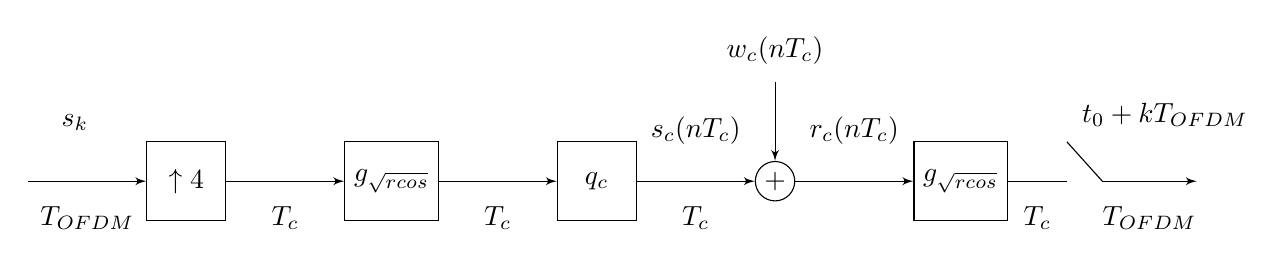
\begin{tikzpicture}[auto,>=latex']
	\tikzstyle{block} = [draw, rectangle, minimum height=1cm, minimum width=1cm]
	
	\node [coordinate, label={[label distance=0.6cm]60:$s_k$}] (start) {};
	\node [block, right = 1.5cm of start] (intpl){$\uparrow 4$};
	\node [coordinate, right = 0.75 cm of intpl] (c1) {};
	\node [block, right = 1.5cm of intpl] (imp){$g_{\sqrt{rcos}}$};
	\node [block, right = 1.5cm of imp] (qc){$q_c$};
	
	\node [draw, circle,minimum size=0.5cm,inner sep=0pt, right = 1.5cm of qc] (sum1){$+$};
	\node [coordinate, right = 0.75cm of imp] (c2) {};
	
	\node [coordinate, label={[label distance=0.1cm]90:$w_c(nT_c)$}, above = 1cm of sum1] (wgn) {};
	
	\node [block, right = 1.5cm of sum1] (matchedf){$g_{\sqrt{rcos}}$};
	\node [coordinate, right = 0.75 cm of matchedf] (c0) {};
	\node [coordinate, above = 0.5 cm of c0, label={[label distance=0.1cm]45:$t_0 + kT_{OFDM}$} ] (c1) {};

	\node [coordinate, right = 1.2cm of matchedf] (c2) {};

	\node [coordinate, right = 1.2cm of c2] (end) {};
	
	\draw [->] (start) --node[label={[label distance=0.2cm]270:$T_{OFDM}$}]{} (intpl);
	\draw [->] (intpl) --node[label={[label distance=0.2cm]270:$T_c$}]{} (imp);
	\draw [->] (imp) --node[label={[label distance=0.2cm]270:$T_c$}]{} (qc);
	\draw [->] (qc) --node[label={[label distance=0.2cm]270:$T_c$},  label={[label distance=0.1cm]90:$s_c(nT_c)$}]{} (sum1);
	\draw [->] (wgn) --node[]{} (sum1);
	\draw [->] (sum1) --node[label={[label distance=0.1cm]90:$r_c(nT_c)$}]{} (matchedf);
	\draw [-] (matchedf) --node[label={[label distance=0.2cm]270:$T_c$}]{} (c0);
	\draw [-] (c1) --node[]{} (c2);
	\draw [->] (c2) --node[label={[label distance=0.2cm]270:$T_{OFDM}$}]{} (end);

	
	\end{tikzpicture}
	\caption{Model for the OFDM channel of Problem 1.}
	\label{Model_OFDM} 
\end{figure}

\begin{figure}[H]
	\centering
	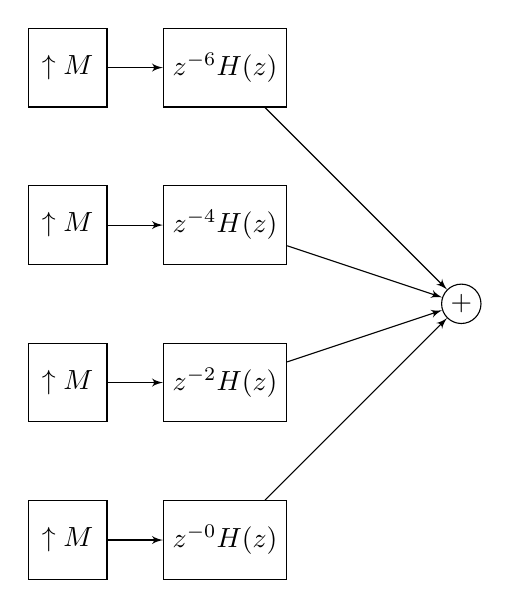
\begin{tikzpicture}[auto,>=latex']
	\tikzstyle{block} = [draw, rectangle, minimum height=1cm, minimum width=1cm]
	
	\foreach \y in {0, 2, ..., 6}
		{ \node [block] (0\y) at (0, \y) {$ \uparrow M$};}
		
	\foreach \y in {0, 2, ..., 6}
	{ \node [block] (1\y) at (2, \y) {$z^{-\y} H(z)$};}
	
	\foreach \y in {0,2,...,6}  
		\draw [->] (0\y)-- (1\y);
		
	\node [draw, circle,minimum size=0.5cm,inner sep=0pt] (sum) at (5,3) {$+$};
		
	\foreach \y in {0,2,...,6}  
	\draw [->] (1\y)-- (sum);
	
	\end{tikzpicture}
\end{figure}

\end{document}